\section{Design}

The CLAS12 DAQ was designed as a pipeline-style, network-based system. The data taking process starts from the front-end components. Those components can have different hardware and software implementations, but have to follow certain requirements to be compatible with the rest of the system. Currently, the front-end components used are commercial VME/VXS crates, commercial Linux servers, and Jefferson Laboratory(JLAB)-designed VXS trigger processor boards. VTPs are installed in all of the VXS crates, but are read out by the DAQ as independent components. All components are running on a 250~MHz clock distributed over OM3-rated parallel optic fibers. The same fiber system is used to distribute thw synchronization reset and trigger signals, and to collect the busy signals from all front-end electronics.

All front-end components are connected to the Event Builder (EB), which is a multi-threaded program running on a multi-core Linux server. Most connections are 1 Gbit ethernet links. For several components that generate significant data rate, 10 Gbit ethernet connection is used.

Complete events are sent to the Event Transfer (ET) System. This multi-threaded program provides a data ring where various data processing programs can be attached to monitor data quality online. It can be run on the same server as the EB, or can be used to create a sequential chain of servers to increase the data processing power.

The last component in the data chain is the Event Recorder (ER). This multi-threaded program receives data from the ET system and records it to the disk. A multi-stream mode is available, that allows several files to be written in parallel to the same or different disk partitions to increase writing performance. The event order in multi-stream mode is preserved. The CLAS12 DAQ system diagram is shown in Fig.~\ref{fig:DAQdiagram}.

\begin{figure}[hbt]
	\centering
	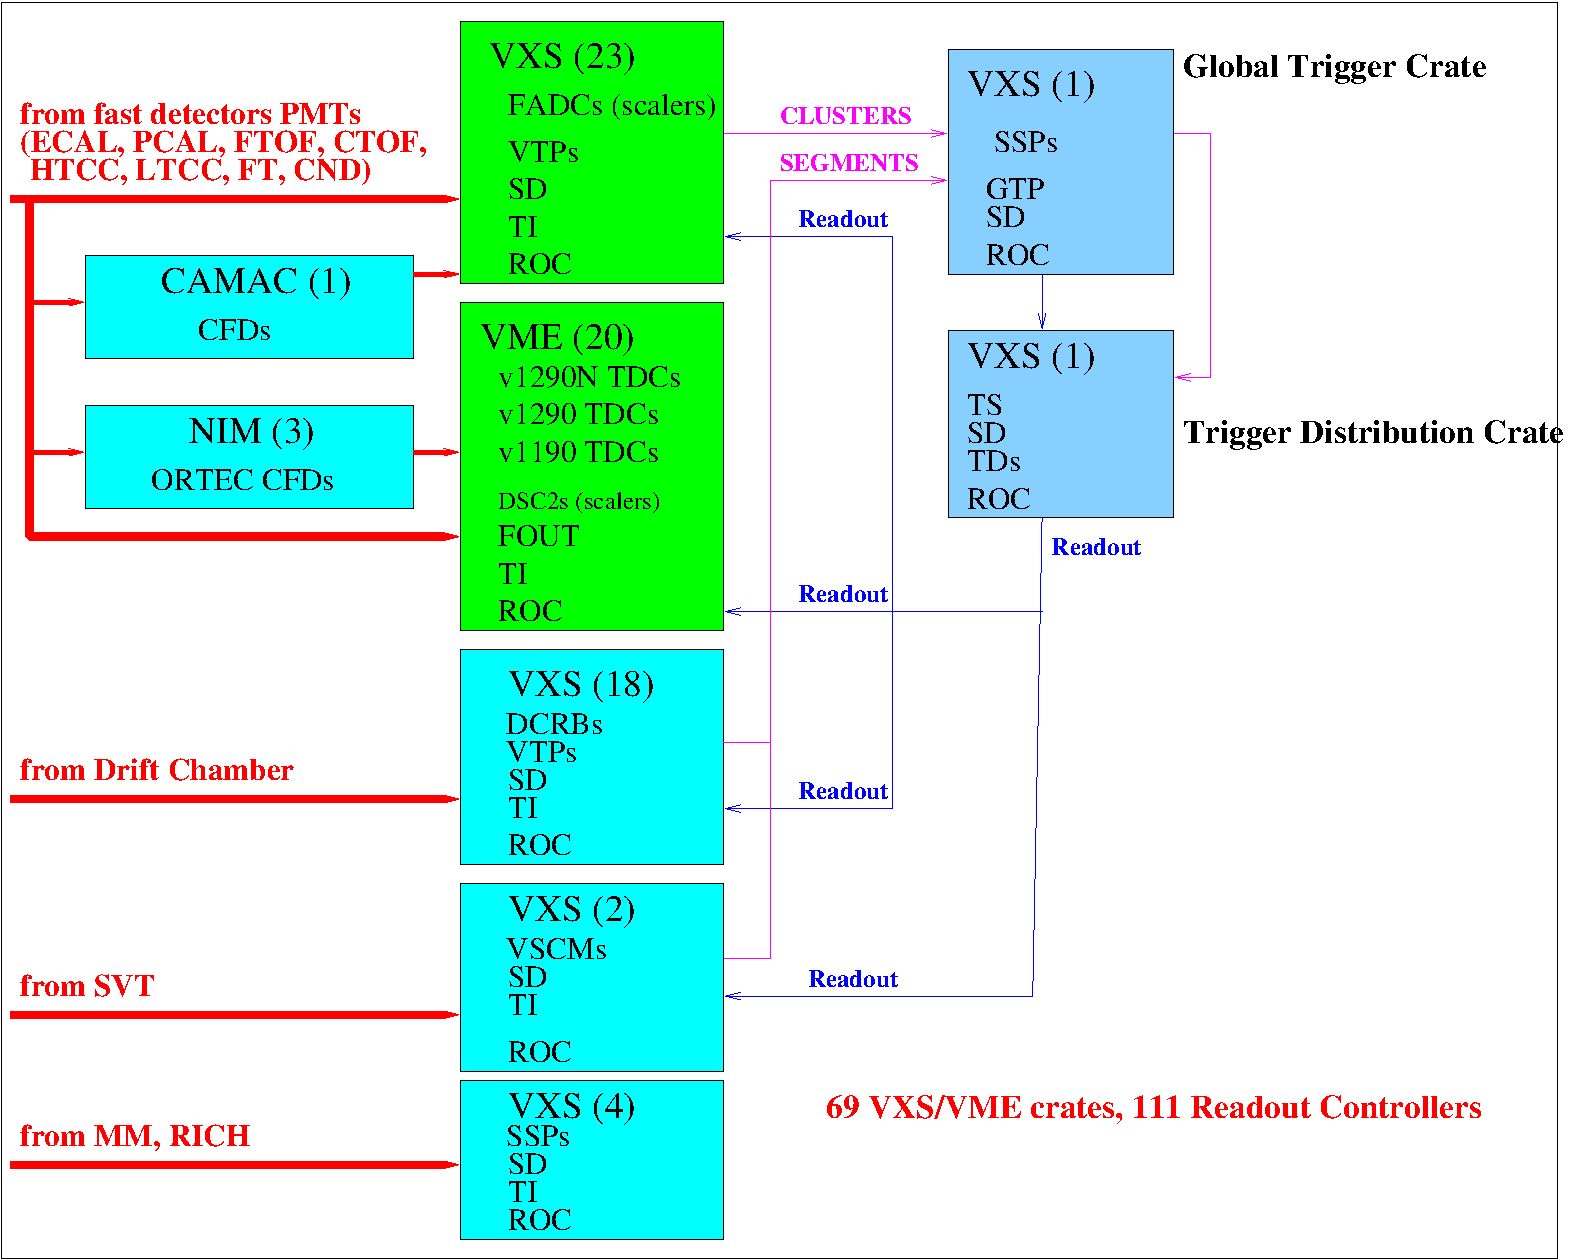
\includegraphics[width=1.0\columnwidth,keepaspectratio]{img/CLAS12_HARDWARE_2.pdf}
	\caption{Diagram of the CLAS12 Data Aquisition System}
	\label{fig:DAQdiagram}
\end{figure}

